\documentclass[11pt]{article}
\usepackage[unicode=true]{hyperref}
\usepackage{multicol}
\usepackage{todonotes}
\usepackage{graphicx}
\usepackage{xcolor}
\usepackage{multirow}
\usepackage{amsmath}

\topmargin=-0.75in
\oddsidemargin=0in
\textwidth=6.5in
\textheight=9.25in
\parindent=0.0in
\parskip=10pt
\linespread{1.0}

\usepackage{marginnote}

% reduce spacing between section headings and set the section font sizes
\usepackage[compact]{titlesec}
\titlespacing{\section}{0em}{0em}{-0.5em}
\titlespacing{\subsection}{0em}{0em}{-0.5em}
\titlespacing{\subsubsection}{0em}{0em}{-0.5em}

\title{Development and Validation of Simulations and Phantoms Mimicking the
    Viscoelastic Properties of Human Liver}
\author{\textbf{Drs.\ Shigao Chen, Ph.D. and Matthew Urban, Ph.D.}\\
        Department of Physiology and Biomedical Engineering\\
        Mayo Clinic \vspace*{0.1in}\\
        \textbf{Dr.\ Stephen McAleavey, Ph.D.}\\
        Department of Biomedical Engineering\\
        University of Rochester \vspace*{0.1in}\\
        \textbf{Dr.\ Jingfeng Jiang, Ph.D.}\\
        Department of Biomedical Engineering\\
        Michigan Technological University \vspace*{0.1in}\\
        \textbf{Dr. Mark L.\ Palmeri, M.D., Ph.D.}\\
        Department of Biomedical Engineering\\
        Duke University}

\date{\textbf{Final Report Submitted:} August 31, 2015}

\begin{document}

\maketitle

\tableofcontents

\section{Project Objectives}

These were the proposed objectives for this funding period:

\begin{description}
    \item[3-Month] Deliverables
        \begin{enumerate}
            \item Recommended VE analysis / reporting method and metrics. 
            \item Validate methods and metrics using the simulations and apply
                to the phantom and potential human data.
        \end{enumerate}

    \item[6-Month] Deliverables
        \begin{enumerate}
            \item Create simulation data matching the Phase II phantom and a
                variety of focal configurations.
            \item Upload simulation data to QIDW\@.
        \end{enumerate}

    \item[12-Month] Deliverables
        \begin{enumerate}
            \item Test and analyze Phase II phantom samples as CIRS/UWM iterate
                on phantom recipes and determine the “best” recipe for
                viscoelastic phantom fabrication and distribution.
            \item Determine the ``best'' viscoelastic material models and
                constants to match the Phase II phantoms and human liver data.
            \item Provide validated open-source alternatives to commercial FEA
                packages. Benchmark results for phase II phantoms will be
                documented and supplied as an integral part of the open-source
                alternatives.
        \end{enumerate}

\end{description}

We have completed all of these objectives, as are detailed in the following
sections.  Section~\ref{sect:ve_analysis} reviews the empirical metrics that
were used to characterize the VE materials used for the Phase II phantom
studies, which were then compared with the human data.
Section~\ref{sect:digital_phantoms} describes the elastic and viscoelastic
digital phantom configuration that were developed, validated and uploaded to
the RSNA QIDW\@.  Section~\ref{sect:open_source} details the open-souce numerical
solvers that were studied as alternative to the commercial solvers used in
Section~\ref{sect:digital_phantoms}, and finally Section~\ref{sect:future_work}
outlines the future efforts for this project in Round V funding.


\section{Viscoelastic Material Analysis Metrics}\label{sect:ve_analysis}

The System Dependency and Phantoms Task Force identified that ``simple'',
analytic viscoelastic material models, such as Voigt and Maxwell materials,
inadequately capture the phase velocity trends measured across the energetic
frequency ranges associate with liver shear wave speed characterization.
Instead of using an analytic VE material model, we proposed characterizing the
phantoms using a linear dispersion model of the form

\begin{equation}
c(f) = c_0 + \frac{dc}{df} f.
\end{equation}

This linear model was fit to the 2D Fourier transform of axial velocity data
over a frequency range of 100--400 Hz, and two metrics were used to
characterize the viscoelasticity of materials:

\begin{enumerate}
    \item Phase velocity at 200 Hz ($c_{200}$), and
    \item Line phase velocity slope from 100--400 Hz ($\frac{dc}{df}$).
\end{enumerate}

This model was applied to human data in patients with liver
fibrosis~\cite{Palmeri2011} (Figure~\ref{fig:phantom_liver_scatter_plot}) to
establish a range of realistic linear dispersion VE material values for healthy
through advanced fibrosis liver health.  The 2D Fourier transform data were
processed using the methods described in~\cite{Nightingale2015,Bernal2011}.  The
data were also validated using human data acquired using a Philips shear wave
imaging system~\cite{Chen2012a}.  

Two important frequency analysis points should be noted:
\begin{enumerate}
    \item The choice of frequency range from 100--400 Hz was chosen based on
        empirical studies of the Duke human data and should not be considered a
        universal recommendation across different imaging systems and clinical
        targets.  Other choices for estimating a linear phase velocity slope
        could include a fixed frequency range about the most energetic center
        frequency or an adaptive frequency range based on each dataset.  

    \item The peak phase velocity data in k-space can be strongly influenced by
        the choice of windowed spatial and temporal shear wave velocity
        data~\cite{Harris1978}.  Inclusion of shear wave data in or adjacent to
        the acoustic radiation force excitation can introduce diffraction
        effects that can significantly skew the frequency analysis of the
        propagating shear waves.
\end{enumerate}

\begin{figure}[htb!]
    \centering
    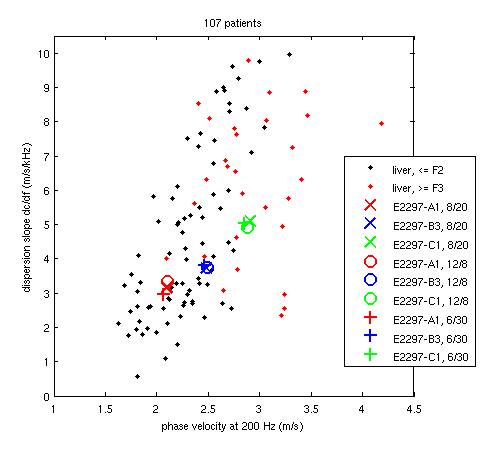
\includegraphics[width=0.75\linewidth]{phantom_liver_scatter_plot.png}
    \caption{Scatter plot comparing mechanical properties of liver (black, red
        dots) in 107 patients with measurements from the CIRS E2297-A1, B3, and
        C1 phantoms made on August 20, 2014 (X’s), December 8, 2014 (O’s), and
        June 30, 2015 (+’s). Points are plotted as a function of (200 Hz) and
        $\frac{dc}{df}$ from a linear dispersion model from 100--400 Hz.}
\label{fig:phantom_liver_scatter_plot}
\end{figure}


\begin{figure}[htb!]
    \centering
    \begin{tabular}{c}
        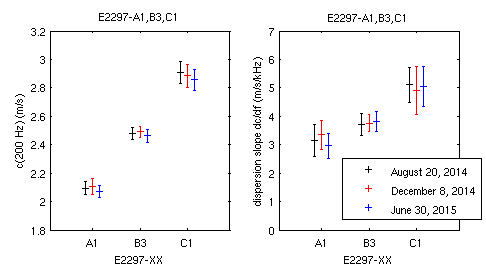
\includegraphics[width=0.75\linewidth]{figs/phase2_longitudinal_stability.png} \\
        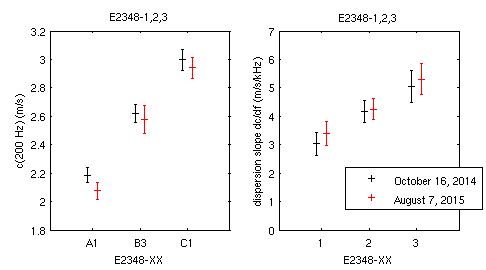
\includegraphics[width=0.75\linewidth]{figs/phaseIIset2_temporal_stability.png} \\
    \end{tabular}
    \caption{Results for the quantities $c_{200}$ (left) and dispersion slope
        $\frac{dc}{df}$ (right) for phantoms [TOP ROW] E2297-A1, B3, and C1
        from measurements made on August 20, 2014 (black), December 8, 2014
        (red), and June 30, 2015 (blue) and [BOTTOM ROW] E2348-1, -2, and -3
        from October 16, 2015 and August 07, 2015. The data points represent
        the mean $\pm$ standard deviation from 16 measurements in each
        phantom.} \label{fig:phase2_longitudinal_stability}
\end{figure}



\section{Digital Phantoms}\label{sect:digital_phantoms}

\subsection{Elastic Materials}
The first-phase of digital phantoms focused on ``simple'' elastic material
formulations with different focal configurations and stiffnesses to evaluate
shear wave speed reconstruction accuracy and precision without viscosity as a
confounding variable.

A nominal curvilinear array configuration was chosen for all of the simulations
(Table~\ref{table:curvilinear}).

\begin{table}[htb!]
    \centering
    \caption{Simulated Curvilinear Array Configuration}
    \begin{tabular}{|l|l|}
    \hline
    Radius of Curvature & 60 mm \\
    Element Height & 14 mm \\
    Element Pitch & 0.477 mm (0.007 mm kerf) \\
    Center Frequency & 3.0 MHz \\
    Fractional Bandwidth & 100\% \\
    Elevation Focus & 50 mm \\
    \hline
    \end{tabular}
\label{table:curvilinear}
\end{table}

The acoustic radiation force excitation was simulated with several focal
configurations (Table~\ref{table:arf}).

\begin{table}[htb!]
    \centering
    \caption{Acoustic Radiation Force Focal Configurations}
    \begin{tabular}{|l|l|}
    \hline
    Frequency & 3.0 MHz \\
    F/\# & [2 ,3.5] \\
    Excitation Durations & [500, 1000] cycles \\
    Focal Depths & [30, 50 70] mm \\
    \hline
    \end{tabular}
\label{table:arf}
\end{table}

Field II~\cite{Jensen1992} was used to simulate the acoustic intensity
associated with the different acoustic radiation force transmit conditions.
The material was acoustically modeled as linear with a constant acoustic
attenuation of 0.45 dB/(cm $\cdot$ MHz).  The acoustic intensity was mapped at
locations in the finite element meshes and the radiation force was either
applied as a point load~\cite{Palmeri2005} at each nodal location or a body
force across elements.

Different elastic material properties were simulated for each of the different
acoustic radiation force focal configurations (Table~\ref{table:elastic}).

\begin{table}[htb!]
    \centering
    \caption{Elastic Material Properties}
    \begin{tabular}{|l|l|}
    \hline
    Poisson's Ratio & 0.495 \\
    Young's Moduli &  [1.0, 2.0, 5.0, 10.0] kPa \\
    \hline
    \end{tabular}
\label{table:elastic}
\end{table}

The finite mesh boundaries were either simulated having perfect matching layers
or infinite elements to reduce artifacts associated with compression and shear
wave reflections back into the regions of interest.  Different mesh densities
were also studied to evaluate numerical accuracy; ultimately a uniform node
spacing of 0.167 mm was used for the digital phantoms.

All of the model configuration scripts for LS-DYNA and ABAQUS have been uploaded to GitHub:

\url{https://github.com/RSNA-QIBA-US-SWS/QIBA-DigitalPhantoms/tree/master/dyna}\\
\url{https://github.com/RSNA-QIBA-US-SWS/QIBA-DigitalPhantoms/tree/master/abaqus}

All of the digital phantom data has been saved in Matlab format and uploaded as
a single archive to QIDW:

\url{http://qidw.rsna.org/community/14}:\verb+US-SWS-Digital-Phantoms -> Public ->+\\
\verb+Elastic Digital Phantoms -> ElasticDigitalPhantomDataMesh0p167mm.zip+

A comprehensive comparison of LS-DYNA and ABAQUS results has been
performed~\cite{Bernal2011}, and the corresponding code to process the data are
available on GitHub:

\url{https://github.com/RSNA-QIBA-US-SWS/QIBA-DigitalPhantoms/tree/master/results}

\subsection{Viscoelastic Materials}
Viscoelastic digital phantoms have been created to more faithfully represent
the known viscous properties of healthy and diseased liver tissue
(Figure~\ref{fig:phantom_liver_scatter_plot}).  Given the large parametric
space of focal / excitation configurations in the elastic digital phantoms, we
restricted the viscoelastic phantoms to three representative parameter sets
that closely match the CIRS Phase II phantoms
(Figure~\ref{fig:phantom_liver_scatter_plot}).  The viscoelastic parameters
were numerically defining a shear relaxation model of the form:
\begin{equation}
    G(t) = G_\infty + (G_0 - G_\infty)e^{-\beta t}.
\label{eqn:shear_relaxation}
\end{equation}
Figure~\ref{fig:ve_data} shows the k-space representations of the spatial and
temporal frequency content arising from a test, axisymmetric Gaussian
excitation, with the associated phase velocity at 200 Hz, and the linear phase
slope from 100--400 Hz.  Table~\ref{table:ve_data} shows how these phase
velocity metrics compare to theoretical values, where the 200 Hz phase
velocities are all $<$5\% overestimation compared to theory, and the phase
velocity slopes are roughly within 10\% of the theoretical slopes.

\begin{figure}[htb!]
    \centering
    \begin{tabular}{c}
        $G_0$ = 10.0 kPa, $G_\infty$ = 2.0 kPa, $\beta$ = 6666.7 s$^{-1}$\\
        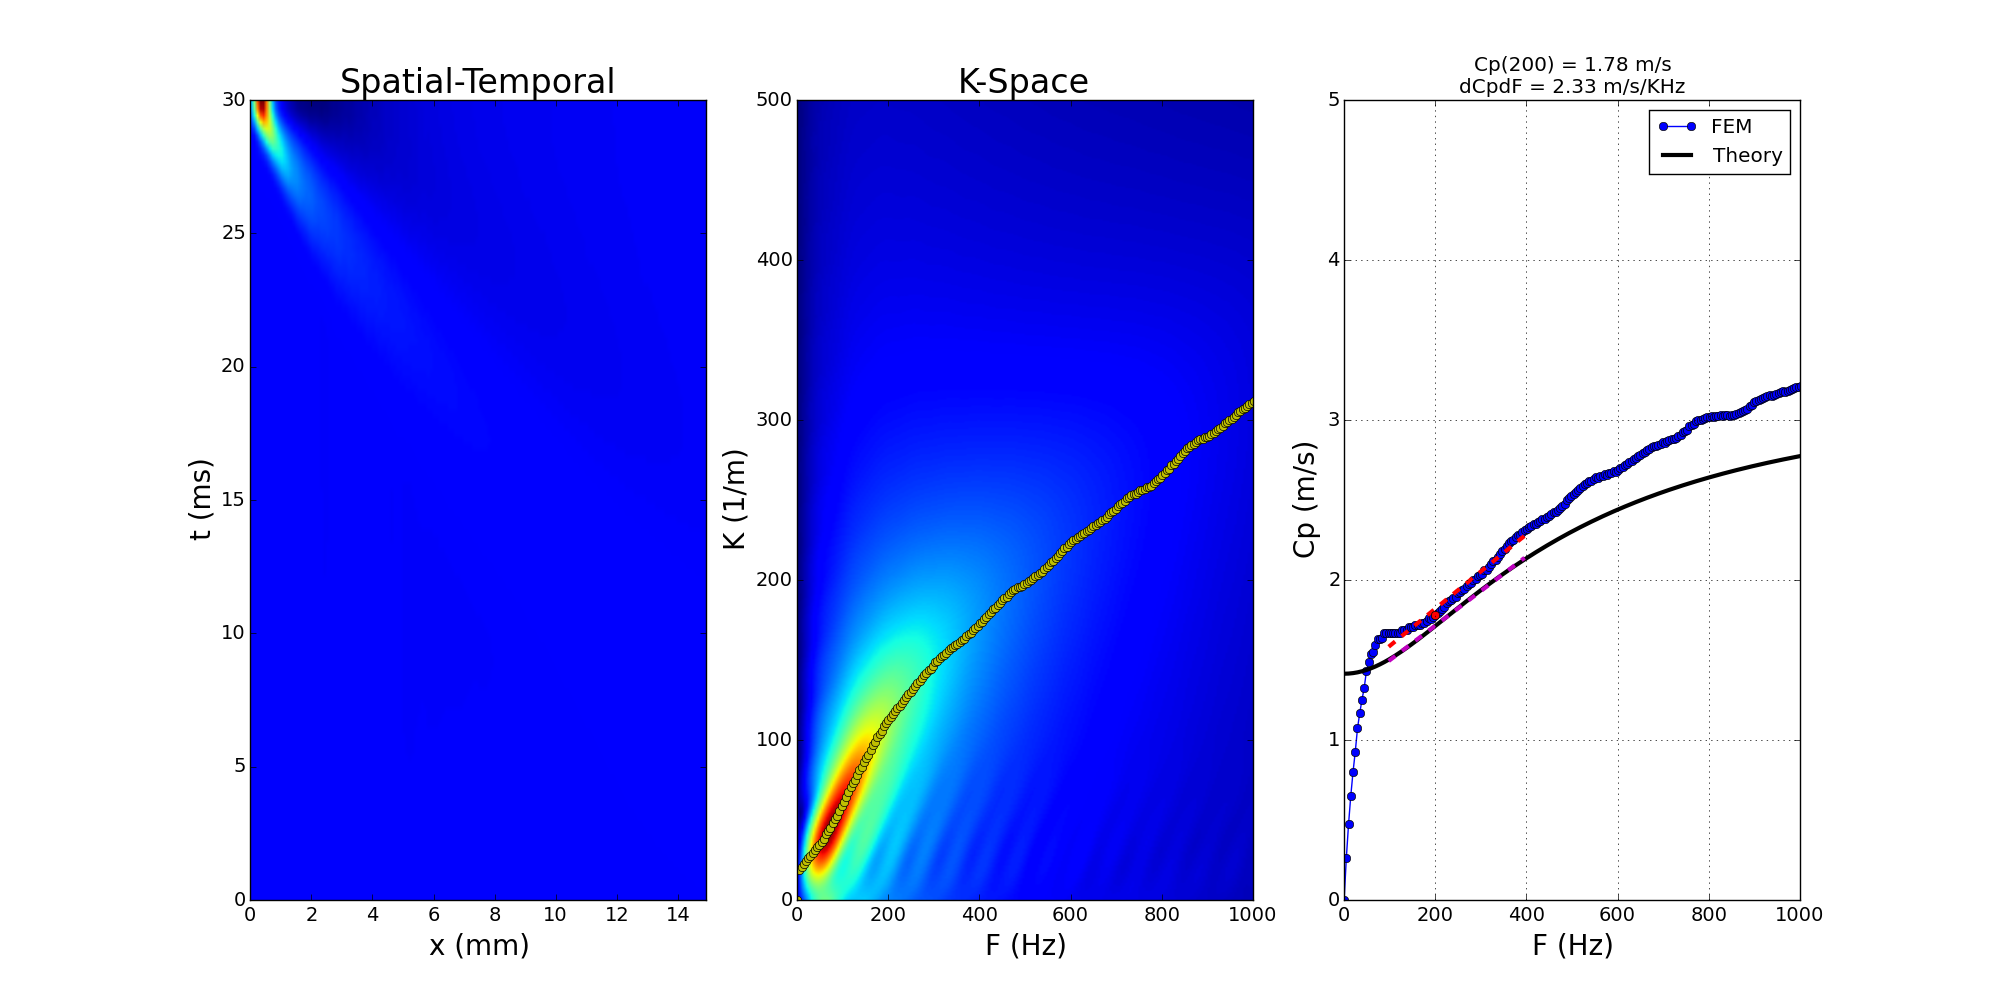
\includegraphics[width=0.75\linewidth]{figs/G010kPa_GI2kPa_BETA6667.png}\\
        $G_0$ = 15.0 kPa, $G_\infty$ = 4.0 kPa, $\beta$ = 5500.0 s$^{-1}$\\
        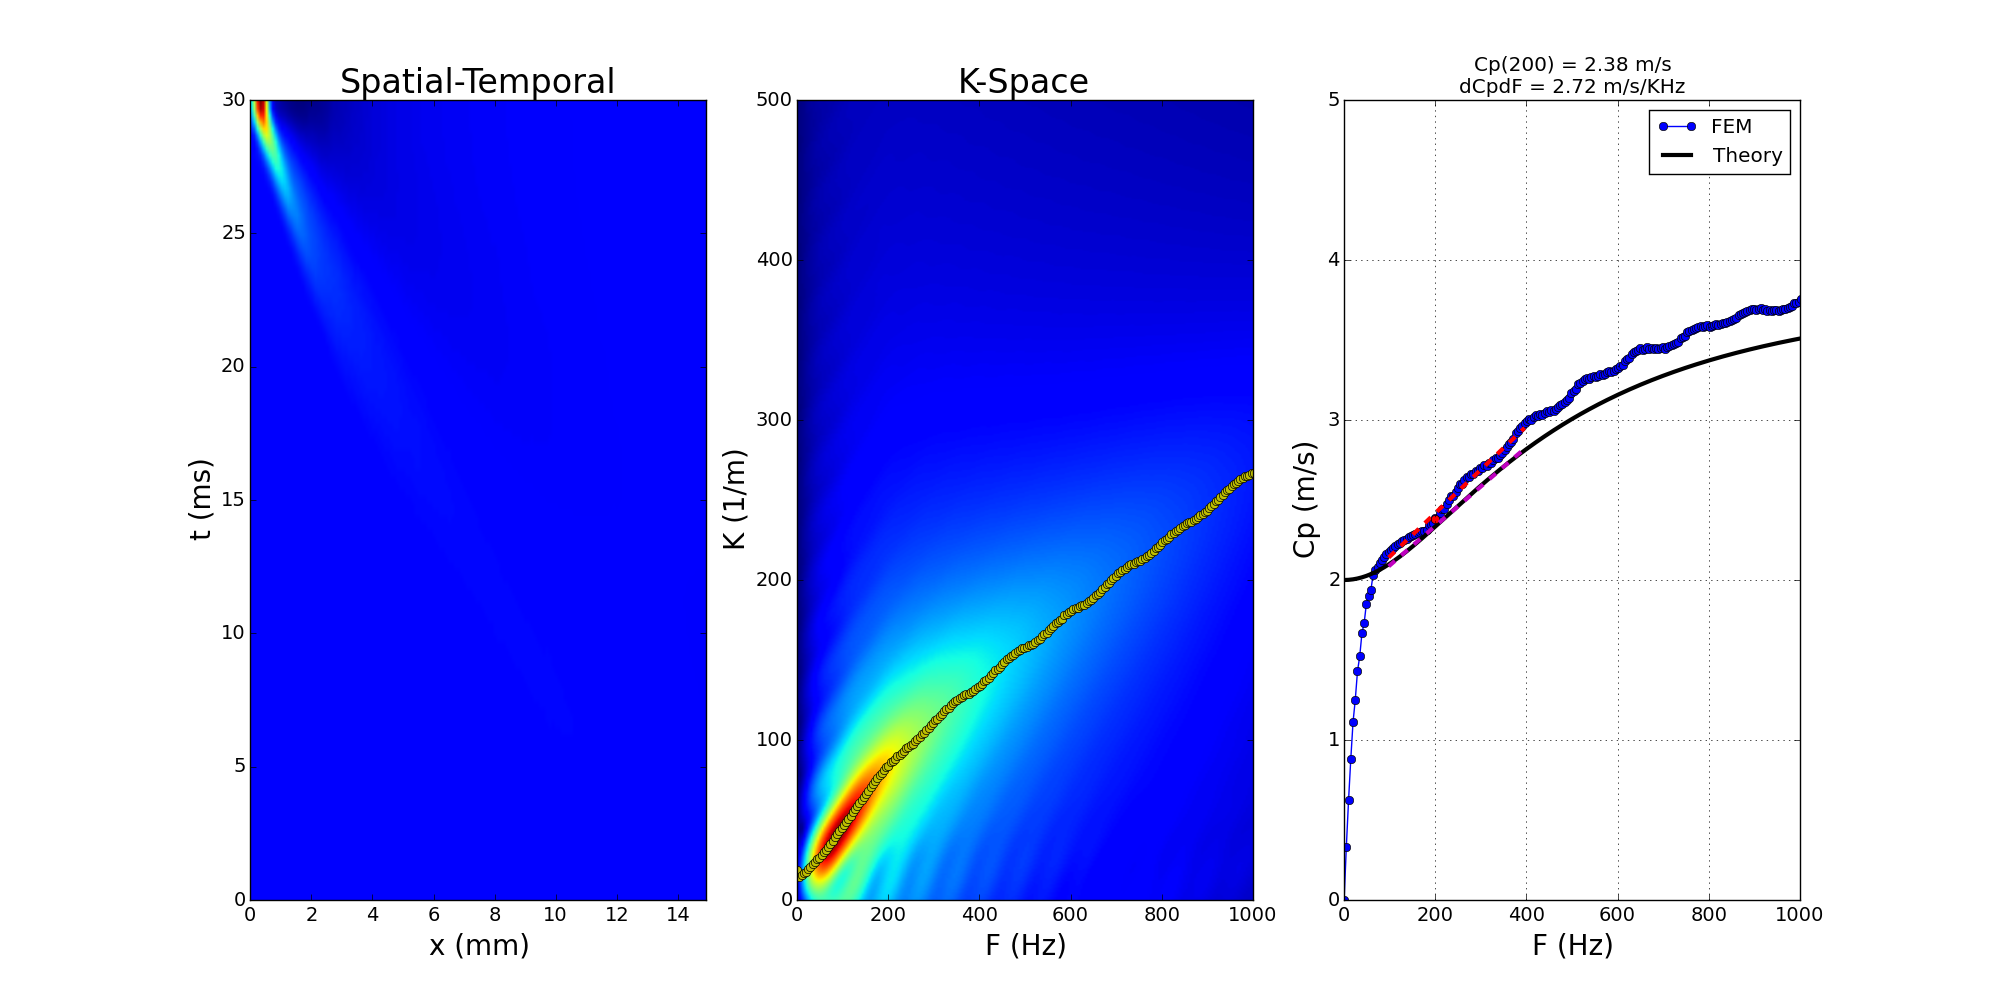
\includegraphics[width=0.75\linewidth]{figs/G015kPa_GI4kPa_BETA5500.png}\\
        $G_0$ = 20.0 kPa, $G_\infty$ = 4.0 kPa, $\beta$ = 4000.0 s$^{-1}$\\
        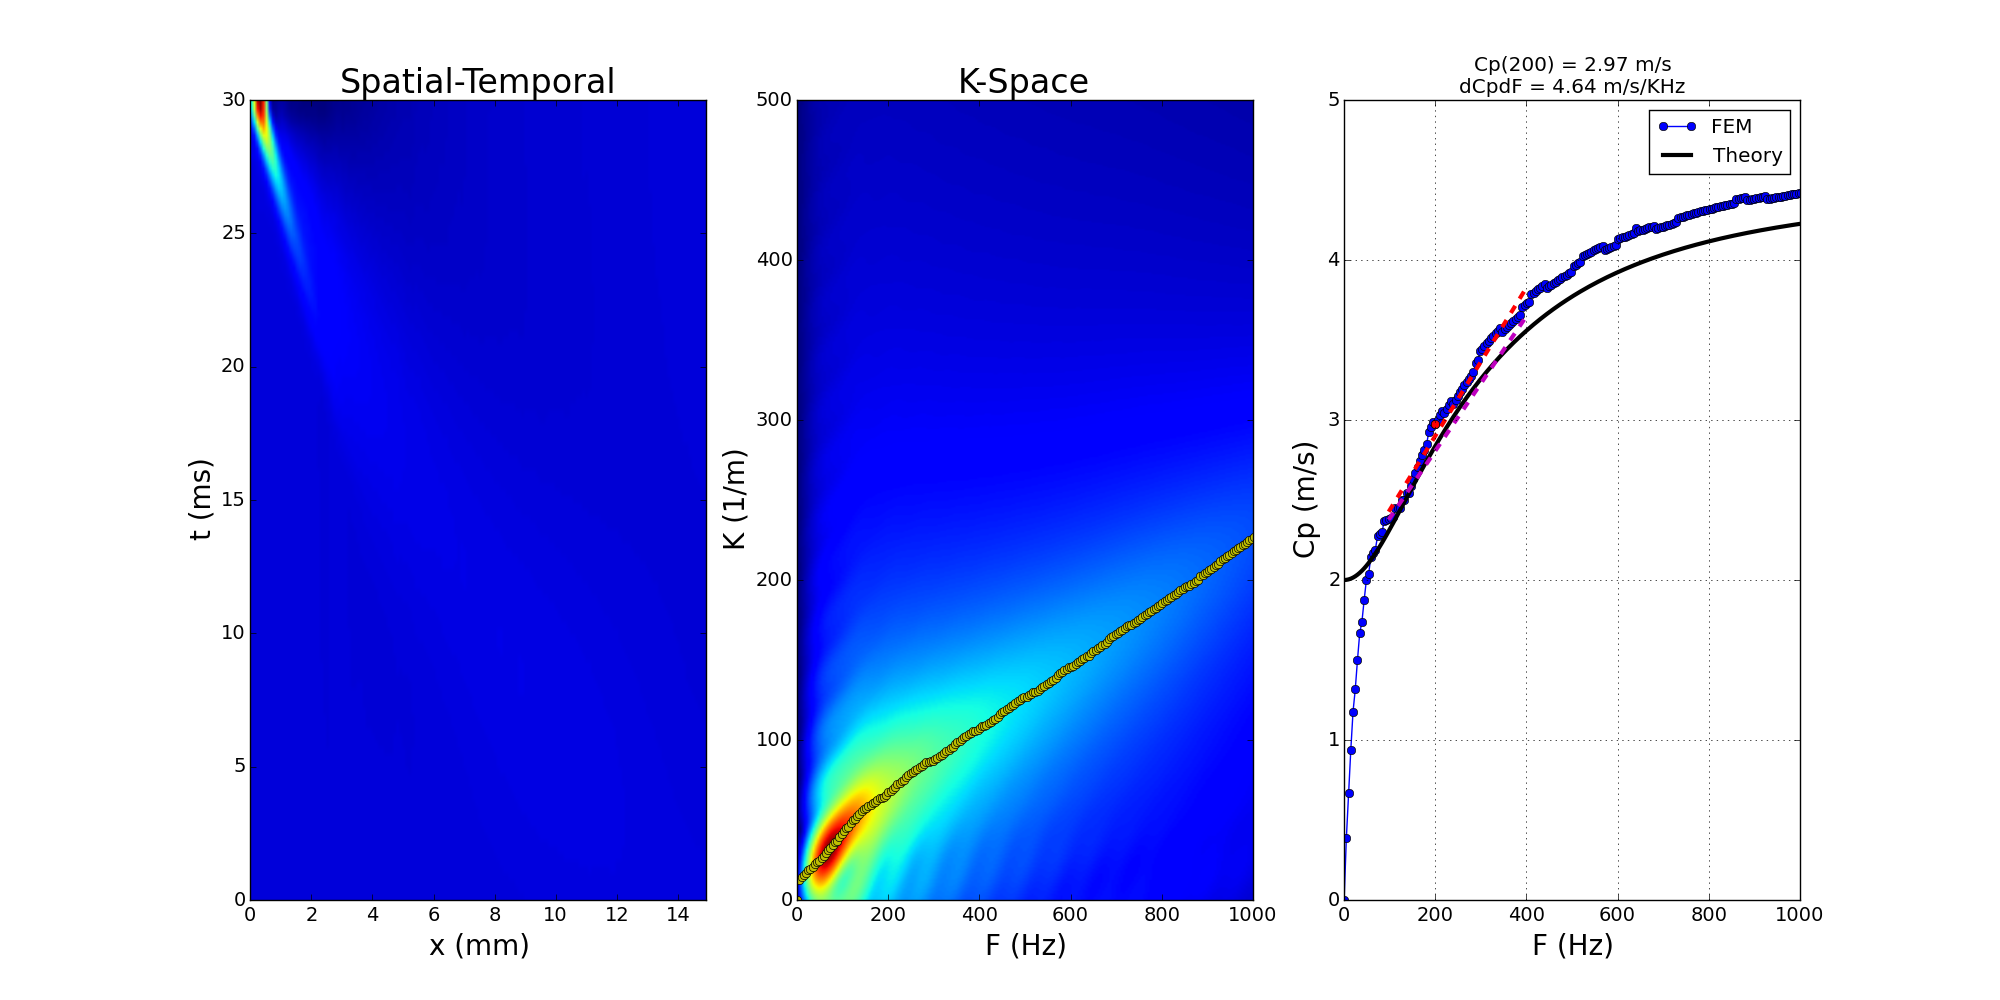
\includegraphics[width=0.75\linewidth]{figs/G020kPa_GI4kPa_BETA4000.png}\\
    \end{tabular}
    \caption{Representative k-space and phase velocity reconstructions 3
        viscoelastic materials that resemble the CIRS Phase II phantoms
        (Figure~\ref{fig:phantom_liver_scatter_plot}).}
\label{fig:ve_data}
\end{figure}

\begin{table}[htb!]
    \centering
    \caption{Viscoelastic material phase velocity metrics compared to theory.
        The phase velocity was calculated at 200 Hz, and the phase velocity
        slope was calculated from 100--400 Hz.  Percent error deviation between
        the FEM-derived metric and the theory are shown in parentheses.}
    \begin{tabular}{|c|c|c|c|c|c|c|}
    \hline
    \multirow{2}{*}{$G_0$ (kPa)} & \multirow{2}{*}{$G_\infty$ (kPa)} & \multirow{2}{*}{$\beta$ (s$^{-1}$)} & \multicolumn{2}{c|}{$c$ (200 Hz, m/s)} & \multicolumn{2}{c|}{$\frac{dc}{df}$ ((m/s)/Hz)} \\ \cline{4-7}
            & & & Theory & FEM & Theory & FEM \\ 
            \hline
            10.0 & 2.0 & 6666.7 & 1.71 & 1.78 (+4.1\%) & 2.16 & 2.33 (+7.9\%) \\ \hline
            15.0 & 4.0 & 5500.0 & 2.33 & 2.38 (+2.1\%) & 2.47 & 2.72 (+10.1\%) \\ \hline
            20.0 & 4.0 & 4000.0 & 2.84 & 2.97 (+4.6\%) & 4.21 & 4.64 (+10.2\%) \\
    \hline
    \end{tabular}
\label{table:ve_data}
\end{table}

These viscoelastic material formulations were then numerical solved for
different focal / excitation configurations, as was done for the elastic
digital phantoms (Tables~\ref{table:curvilinear} \&~\ref{table:arf}).  The
viscoelastic digital phantom data has also be uploaded to the QIDW
US-SWS-Digital-Phantoms community.

There are a number of areas of data processing and analysis that could lead to
differences in estimated values of shear wave velocity, particularly for
viscoelastic materials. For the purposes of analysis of the viscoelastic
phantoms, a Fourier-based analysis is typically performed. As the data is
discrete, fast Fourier transforms (FFTs) are applied to the data to transform
the spatiotemporal data to the Fourier domain (commonly referred to k-space).
Different groups apply different spatial and temporal windows to the data
before the FFTs are applied which can alter the subsequent data analysis.

Once the k-space distribution is established, there are also varying methods
for analyzing the shear wave velocity dispersion. Different search strategies
are employed to obtain the shear wave velocity values including peak detection
in the k-space or a Radon sum approach to name two. Once the shear wave phase
velocities are identified, different models can be fit to the data including a
Voigt model or a linear model that has a specific intercept and slope over a
given bandwidth. The choice of the bandwidth can also affect the results.

With these variables associated with the processing, a set of preferred or
recommended practices has yet to be established but will be the focus of future
work.


\section{Open-Source Numerical Shear Wave Solvers}\label{sect:open_source}

\subsection{FEBio}
Building on Round III effort, Dr. Jiang has extended the FEBio (INSERT FOOTNOTE
URL) model of elastic shear wave propagation to include viscoelastic media.  An
example FEBio simulation template has been provided in the GitHub repository:

\url{https://github.com/RSNA-QIBA-US-SWS/QIBA-DigitalPhantoms/tree/master/febio}

Below is a comparison of the reconstructed viscoelastic material metrics
reconstructed for the 3 configurations used to generate the viscoelastic
digital phantoms:

INSERT TABLE HERE

It was found during Round III that the lack of a perfect matching layer
boundary condition or any other damping boundary that can simulate a
semi-infinite medium introduced appreciable artifact in the FEBio models.
These boundary condition limitations are still a first-order limitation of
using FEBio as a replacement for the commercial FEA solvers.

\subsection{C-Scan Finite Difference Code}
Dr. McAleavey has developed finite difference code solving shear wave
propagation in C-scan planes in viscoelastic media.  This code has been
optimized to run in a GPGPU environment on a desktop workstation and requires
considerably lower computation overhead than the commercial FEA software
packages used to generate the digital phantom data uploaded to QIDW.

Source code for this finite difference algorithm has been shared in the GitHub
repository:

INSERT HYPERLINK HERE

Below is a comparison of the reconstructed viscoelastic material metrics
reconstructed for the 3 configurations used to generate the viscoelastic
digital phantoms:

INSERT TABLE HERE

This code provides accurate solutions in the C-scan plane, but full volumetric
simulated displacement / velocity data are not yet available using this
approach.  This code will continue to evolve through external funding beyond
the scope of QIBA support.


\section{Future Work}\label{sect:future_work}

We have met all of our Round IV objectives, and we plan to extend our digital
phantom and viscoelastic phantom characterization efforts in Round V as
follows:

\begin{enumerate}
    \item Perform statistical analysis on the Phase II measurment data and
    compare with simulated viscoelastic analyses.
    \item Expand the acoustic radiation force focal configurations to general
    shear waves with different spectral distributions of energy.
    \item Augment the existing visoelastic digital phantoms to have simulated
    raw RF / IQ data for displacement estimation.
    \item Evaluate the impact of attenuation and phase aberration effects on
    acoustic radiation force source distribution on the reconstructed shear
    wave speed.
\end{enumerate}

More details are available in the Round V proposal that was submitted earlier in the year.


\section{Presentations \& Publications}

Work from this project has been presented / published in the past year as follows:

\begin{itemize}
    \item AIUM
    \item ITEC
\end{itemize}

We also plan to submit a manuscript on these modeling methods to an IEEE UFFC
special issue dedicated to different ultrasound simulation and experiment
methodology.  An announcement for this special issue can be found HERE (INSERT
URL).


\section{Acknowledgements}
Special thanks to Drs. Kathy Nightingale and Ned Rouze, and Yufeng Deng, for
their efforts characterizing the CIRS Phase II phantoms and providing the
viscoelastic analysis of these samples.  Special thanks to Bo Qiang for leading
the ABAQUS simulations and providing the thorough analysis with LS-DYNA data
for the elastic simulations, and Jonathan Langdon for development of the
open-source, GPU-accelerated shear wave simulation code.  In addition to the
QIBA funding for this project, this work was also supported by contracts HHSN
268201300071C and HHSF 223201400703P and grants R01 DK092255 and R01 EB002132.


\pagebreak

\section{References Cited}
\renewcommand{\refname}{}
\bibliographystyle{abbrv}
\bibliography{references}


\end{document}
